\documentclass[pdflatex,compress,mathserif]{beamer}

%\usetheme[dark,framenumber,totalframenumber]{ElektroITK}
\usetheme[darktitle,framenumber,totalframenumber]{ElektroITK}

\usepackage[utf8]{inputenc}
\usepackage[T1]{fontenc}
\usepackage{lmodern}
\usepackage[bahasai]{babel}
\usepackage{amsmath}
\usepackage{amsfonts}
\usepackage{amssymb}
\usepackage{graphicx}
\usepackage{multicol}
\usepackage{lipsum}
\usefonttheme[onlymath]{serif}

\newcommand*{\Scale}[2][4]{\scalebox{#1}{$#2$}}%

\setbeamertemplate{caption}[numbered]

\title{METODE NUMERIK}
\subtitle{Solusi Akar-Akar Persamaan Non-Linear}

\author{Mifta Nur Farid}

\begin{document}

\maketitle

\section{Pengantar}

\begin{frame}
	\frametitle{Pengantar}
	\begin{itemize}
		\item Persamaan derajat tinggi dapat berupa polinomial-polinomial atau persamaan-persamaan yang mengandung fungsi radikal dan/atau transendental (trigonometrik dan logaritmik).
		\item Contoh sederhana
		$$ ax^2 + bx + c = 0 $$
		\item Berdasarkan ilmu aljabar, akar-akarnya:
		$$ x = \frac{-b \pm \sqrt{b^2 - 4ac}}{2a} $$
		\item Namun dalam kasus persamaan-persamaan derajat tinggi, metode numerik biasanya hanya satu-satunya cara untuk mendapatkan solusi atau akar-akarnya.
	\end{itemize}
\end{frame}

\begin{frame}
	\frametitle{Sub-CPMK}
	\textbf{Sub Capaian Pembelajaran Mata Kuliah (Sub CPMK):}\\Mahasiswa mampu menentukan akar-akar dari persamaan non linear secara numerik (C3, P2, A2)
\end{frame}

\begin{frame}
	\frametitle{Bahan Kajian}
	\begin{enumerate}
		\item Metode iterasi sederhana;
		\item Metode Newton-Raphson;
		\item Metode bagi dua/ biseksi;
		\item Metode Regula-Falsi;
		\item Metode Secant.
	\end{enumerate}
\end{frame}

\section{Metode Iterasi Sederhana}

\begin{frame}
	\frametitle{Metode Iterasi Sederhana}
	Algoritma metode Iterasi Sederhana
	\begin{enumerate}
		\item Kita atur persamaan yang akan kita cari akar-akarnya sedemikian rupa sehingga variabel berada di sisi kanan. Misalkan persamaannya adalah
		$$ x^2 - 2x - 8 = 0 $$
		dapat kita atur sedemikian rupa sehingga menjadi
		$$ x = 0.5x^2 - 4 $$ atau $$ x = \sqrt{2x+8} $$
		\item Kita asumsikan suatu nilai awalan untuk memulai iterasi pertama, yaitu $x_\text{lama}$
	\end{enumerate}
\end{frame}

\begin{frame}{Metode Iterasi Sederhana}
	\begin{enumerate}
		\setcounter{enumi}{2}
		\item Kita substitusikan nilai $x_\text{lama}$ tadi ke sisi kanan dari persamaan untuk mencari nilai $x_\text{baru}$ di sisi kiri persamaan. Sehingga: $$ x_{\text{baru}} = 0.5(x_\text{lama})^2 - 4 $$
		\item Jika $|x_\text{baru} - x_\text{lama}| > \varepsilon $, maka $x_\text{lama} = x_\text{baru}$.
		\item Ulangi langkah ke-3 dan ke-4 hingga $|x_\text{baru} - x_\text{lama}| \leq \varepsilon $
		\item Jika $|x_\text{baru} - x_\text{lama}|$ semakin besar maka ganti nilai nilai awalan di langkah ke-2 atau ganti bentuk persamaan yang lain.
	\end{enumerate}
\end{frame}

\begin{frame}
	\frametitle{Contoh 1}
	Tentukan akar-akar dari persamaan $$ 2x^2 - 5x + 3 = 0 $$ dengan menggunakan metode iterasi sederhana.
\end{frame}

\begin{frame}
	\frametitle{Solusi Contoh 1}
	\begin{enumerate}
		\item Ubah bentuk persamaannya: $$ x = \frac{2x^2+3}{5} $$ atau $$ x = \sqrt{\frac{5x-3}{2}} $$
	\end{enumerate}
\end{frame}

\begin{frame}
	\frametitle{Solusi Contoh 1}
	\begin{enumerate}\setcounter{enumi}{1}
		\item Asumsikan nilai awalan, misalkan $x = 0$
		\item Hitung nilai $x_{\text{baru}}$ dengan menggunakan persamaan $ x = \frac{2x^2+3}{5} $ yang mana $x$ di sisi kiri adalah $x_{\text{baru}}$ dan $x$ di sisi kanan adalah $x$ nilai awalan. $$ x_{\text{baru}} = \frac{2x^2+3}{5} $$
		\item Kita coba langkah-langkah selanjutnya dengan bantuan excel/ spreadsheet
	\end{enumerate}
\end{frame}

\section{Metode Newton-Raphson}

\begin{frame}
	\frametitle{Metode Newton-Raphson}
	Algoritma metode Newton-Raphson sama dengan metode iterasi sederhana. Hal yang membedakan hanya penggunaan persamaan baru, yaitu $$ x_{\text{baru}} = x - \frac{f(x)}{f'(x)} $$
\end{frame}

\begin{frame}
	\frametitle{Contoh 2}
	Tentukan akar-akar dari persamaan $$ 2x^2 - 5x + 3 = 0 $$ dengan menggunakan metode Newton-Raphson.
\end{frame}

\section{Metode Bagi Dua}

\begin{frame}
	\frametitle{Metode Bagi Dua}
	\begin{center}
		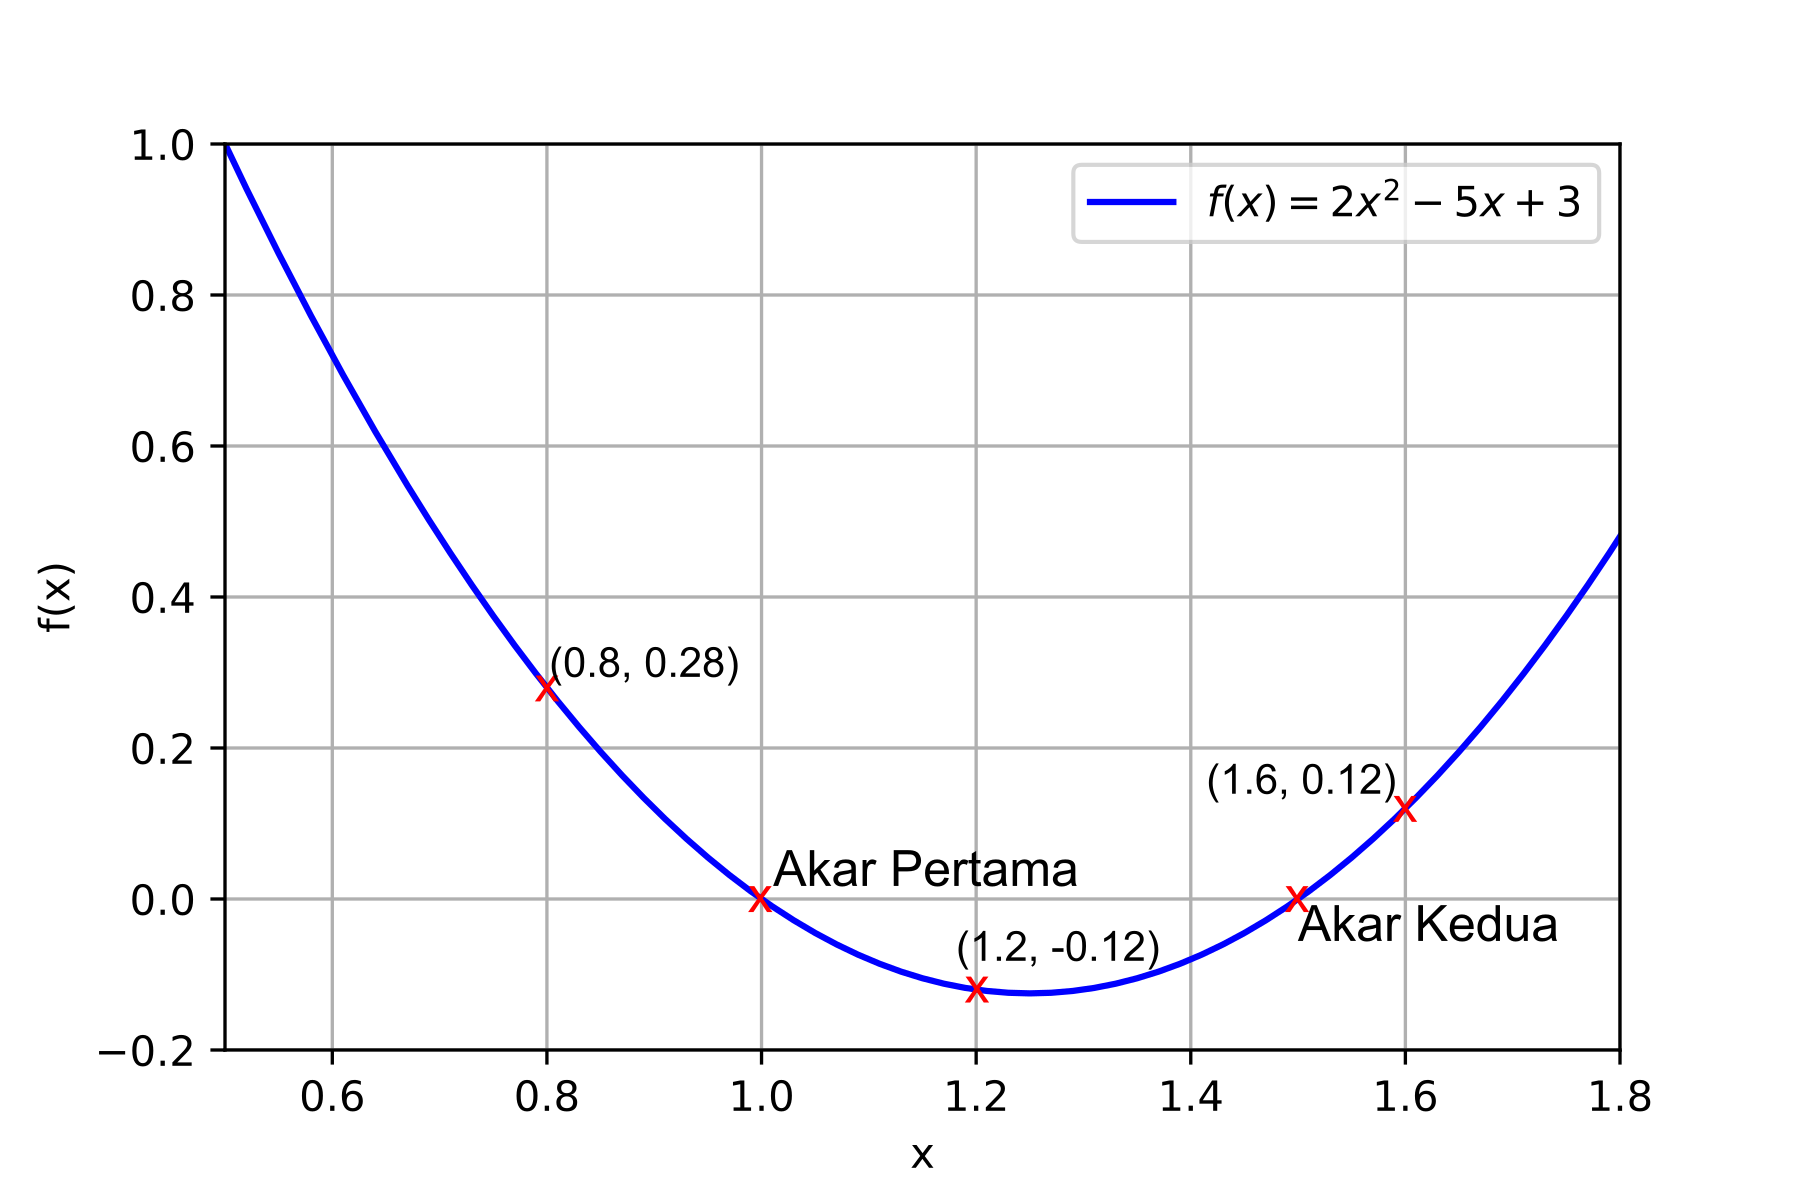
\includegraphics[width=\linewidth]{img/01}
	\end{center}
\end{frame}

\begin{frame}{Metode Bagi Dua}
	\begin{center}
		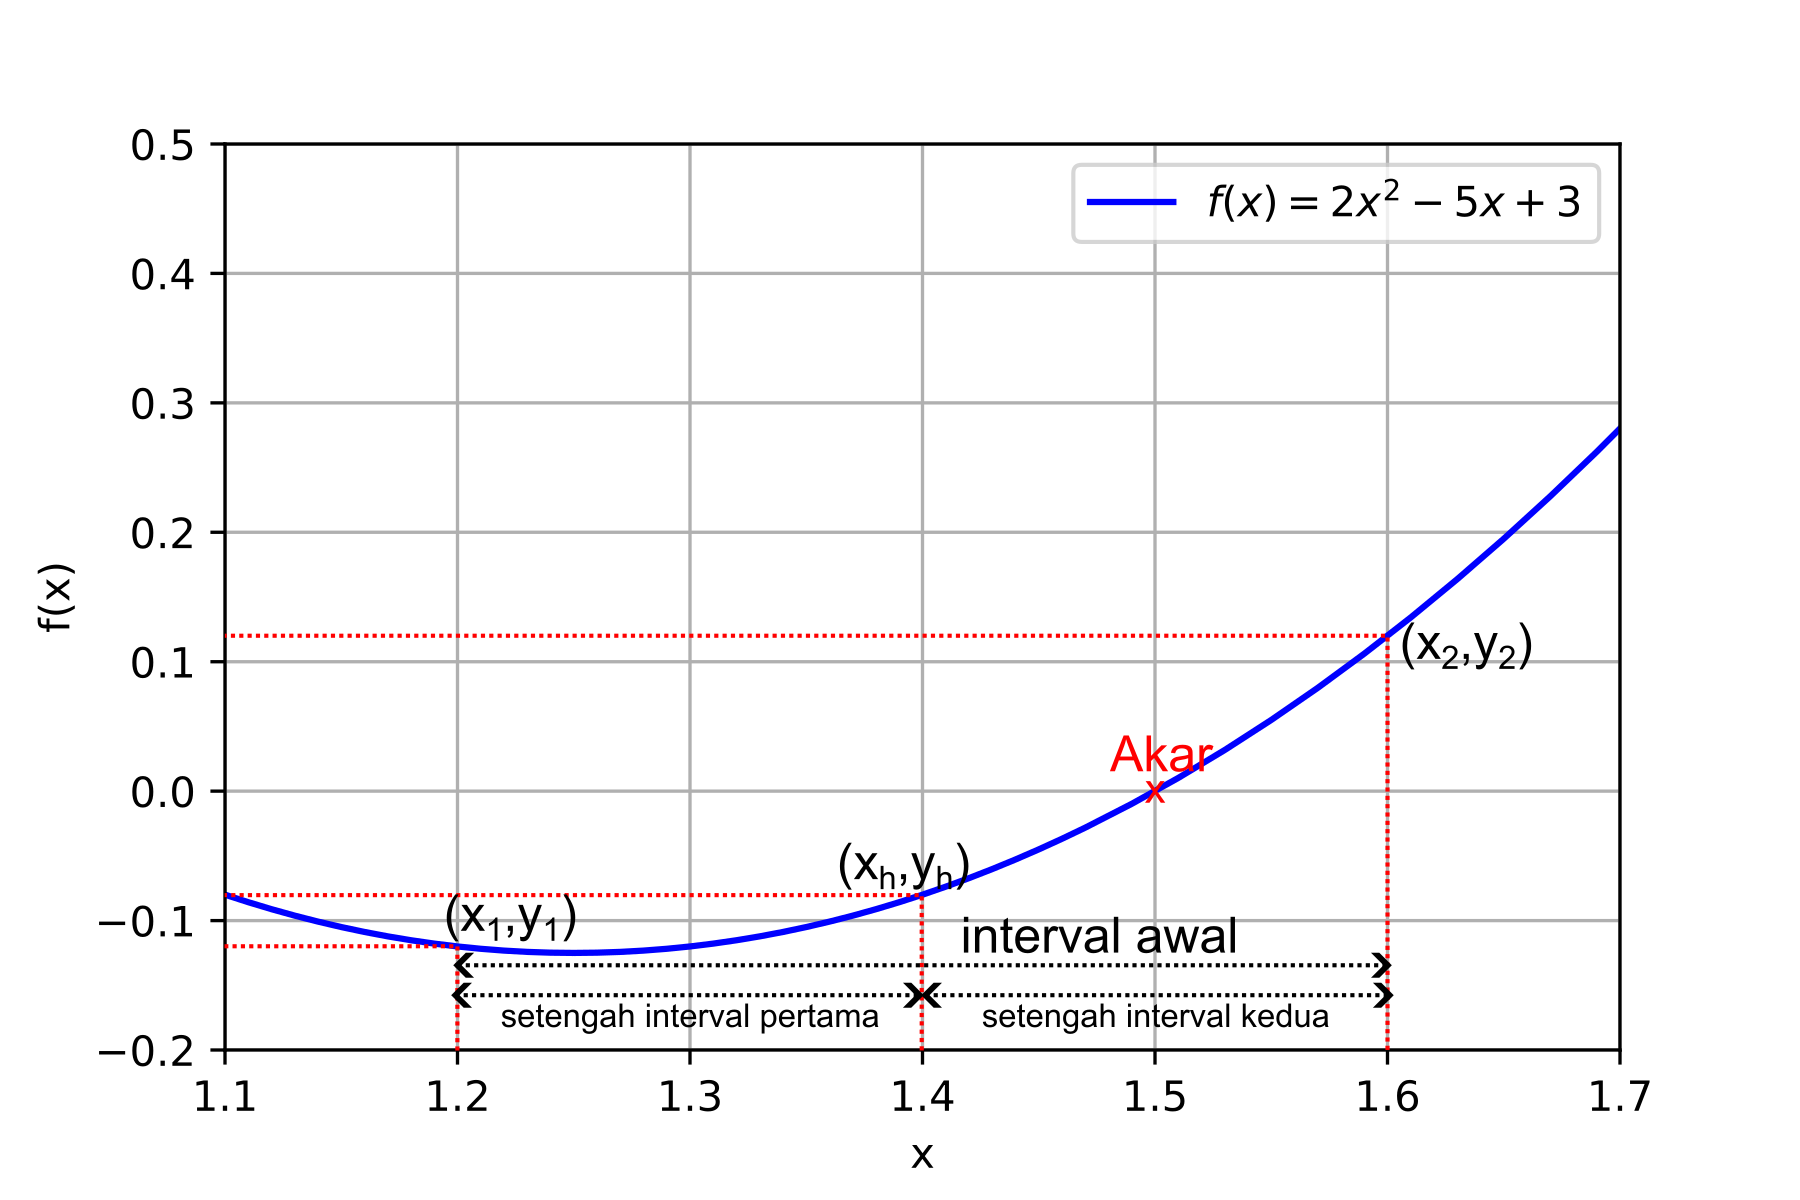
\includegraphics[width=\linewidth]{img/02}
	\end{center}
\end{frame}

\begin{frame}{Metode Bagi Dua}
	Algoritma metode Bagi Dua
	\begin{enumerate}
		\item Masukkan dua nilai awalan ke dalam $ x_1 $ dan $ x_2 $ yang ditengarai akar-akarnya berada di dalam interval dari kedua nilai tersebut.
		\item Hitung $ y_1 $ dan $ y_2 $.
		\item Periksa perbedaan tanda antara $ y_1 $ dan $ y_2 $.
		\item Jika tandanya sama, maka berhenti.
		\item Hitung nilai $ x_h $ yang membagi interval awal menjadi setengah interval sama panjang.
	\end{enumerate}
\end{frame}

\begin{frame}{Metode Bagi Dua}
	\begin{enumerate}
		\setcounter{enumi}{5}
		\item Periksa perbedaan tanda antara $ y_1 $ dan $ y_h $ di setengah interval pertama.
		\item Jika tandanya berlawanan, maka $ x_1 $ dan $ x_2 $ adalah setengah interval pertama.
		\item Jika tandanya sama, maka $ x_1 $ dan $ x_2 $ adalah setengah interval kedua.
		\item Jika nilai $ y_1 $ dan $ y_2 $ mendekati nilai nol, maka tampilkan nilai x dan berhenti.
		\item Jika tidak, maka ulangi langkah ke 5 hingga langkah ke 10.
	\end{enumerate}
\end{frame}

\begin{frame}
	\frametitle{Contoh 3}
	Tentukan akar-akar dari persamaan $$ 2x^2 - 5x + 3 = 0 $$ dengan menggunakan metode bagi dua.
\end{frame}

\section{Metode Regula Falsi}

\begin{frame}
	\frametitle{Metode Regula Falsi}
	\begin{itemize}
		\item Algoritma metode Regula Falsi hampir sama dengan metode Bagi Dua karena kebutuhan terhadap 2 titik.
		\item Hal yang membedakan adalah metode pencarian titik selanjutnya.
		
	\end{itemize}
\end{frame}

\begin{frame}{Metode Regula Falsi}
	\begin{center}
		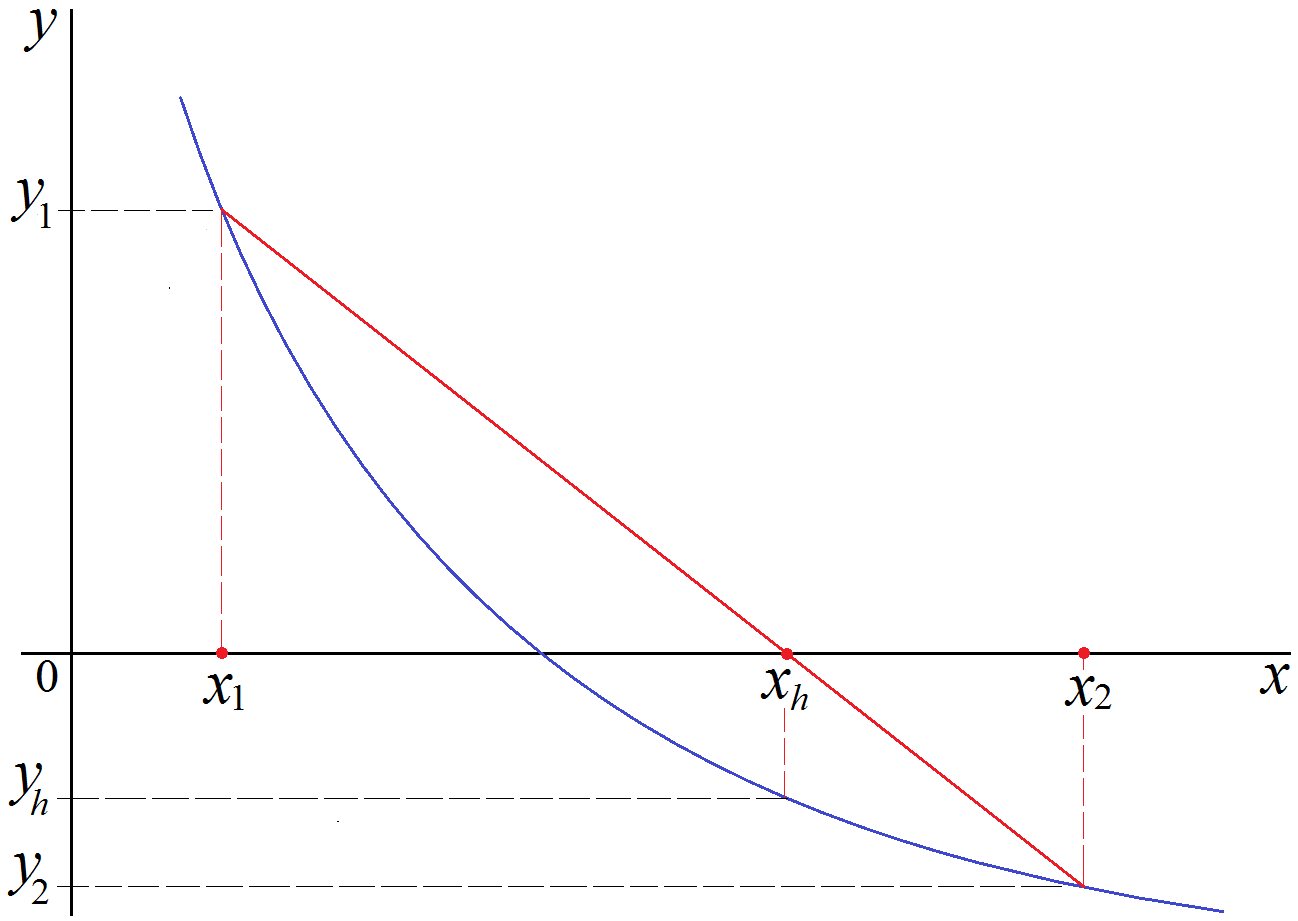
\includegraphics[width=0.7\linewidth]{img/03}
	\end{center}
	$$ \frac{y_2 - y_1}{x_2 - x_1} = \frac{y_2 - 0}{x_2 - x_h} $$
\end{frame}

\begin{frame}{Metode Regula Falsi}
	\begin{center}
		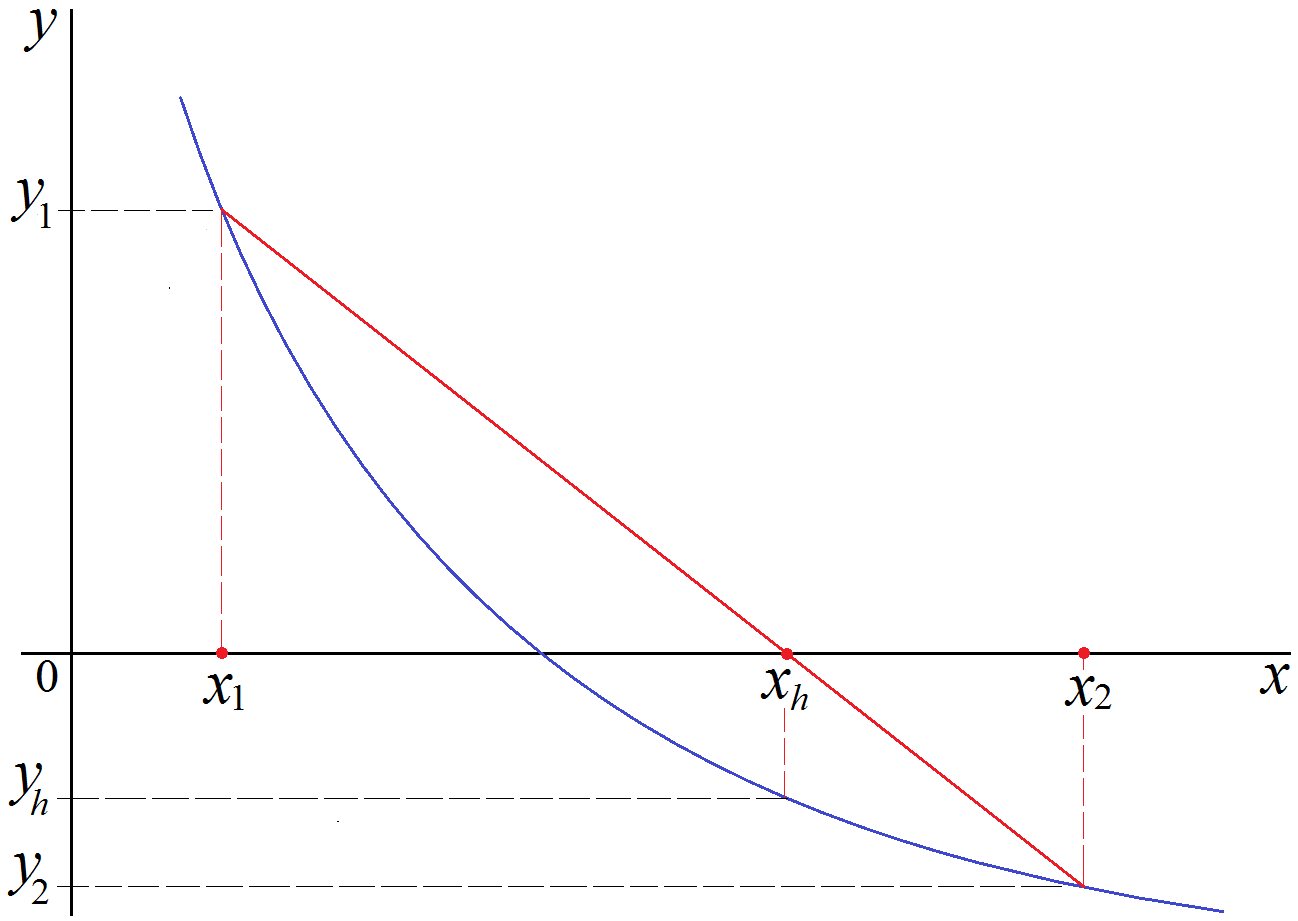
\includegraphics[width=0.7\linewidth]{img/03}
	\end{center}
	$$ x_h = x_2 - \frac{x_2 - x_1}{y_2 - y_1}y_2 $$
\end{frame}

\begin{frame}
	\frametitle{Contoh 4}
	Tentukan akar-akar dari persamaan $$ 2x^2 - 5x + 3 = 0 $$ dengan menggunakan metode Regula Falsi.
\end{frame}

\section{Metode Secant}

\begin{frame}
	\frametitle{Metode Secant}
	\begin{itemize}
		\item Metode Secant hampir sama dengan metode Regula Falsi.
		\item Hal yang membedakan adalah metode pencarian titik selanjutnya.
	\end{itemize}
\end{frame}

\begin{frame}{Metode Secant}
	\begin{center}
		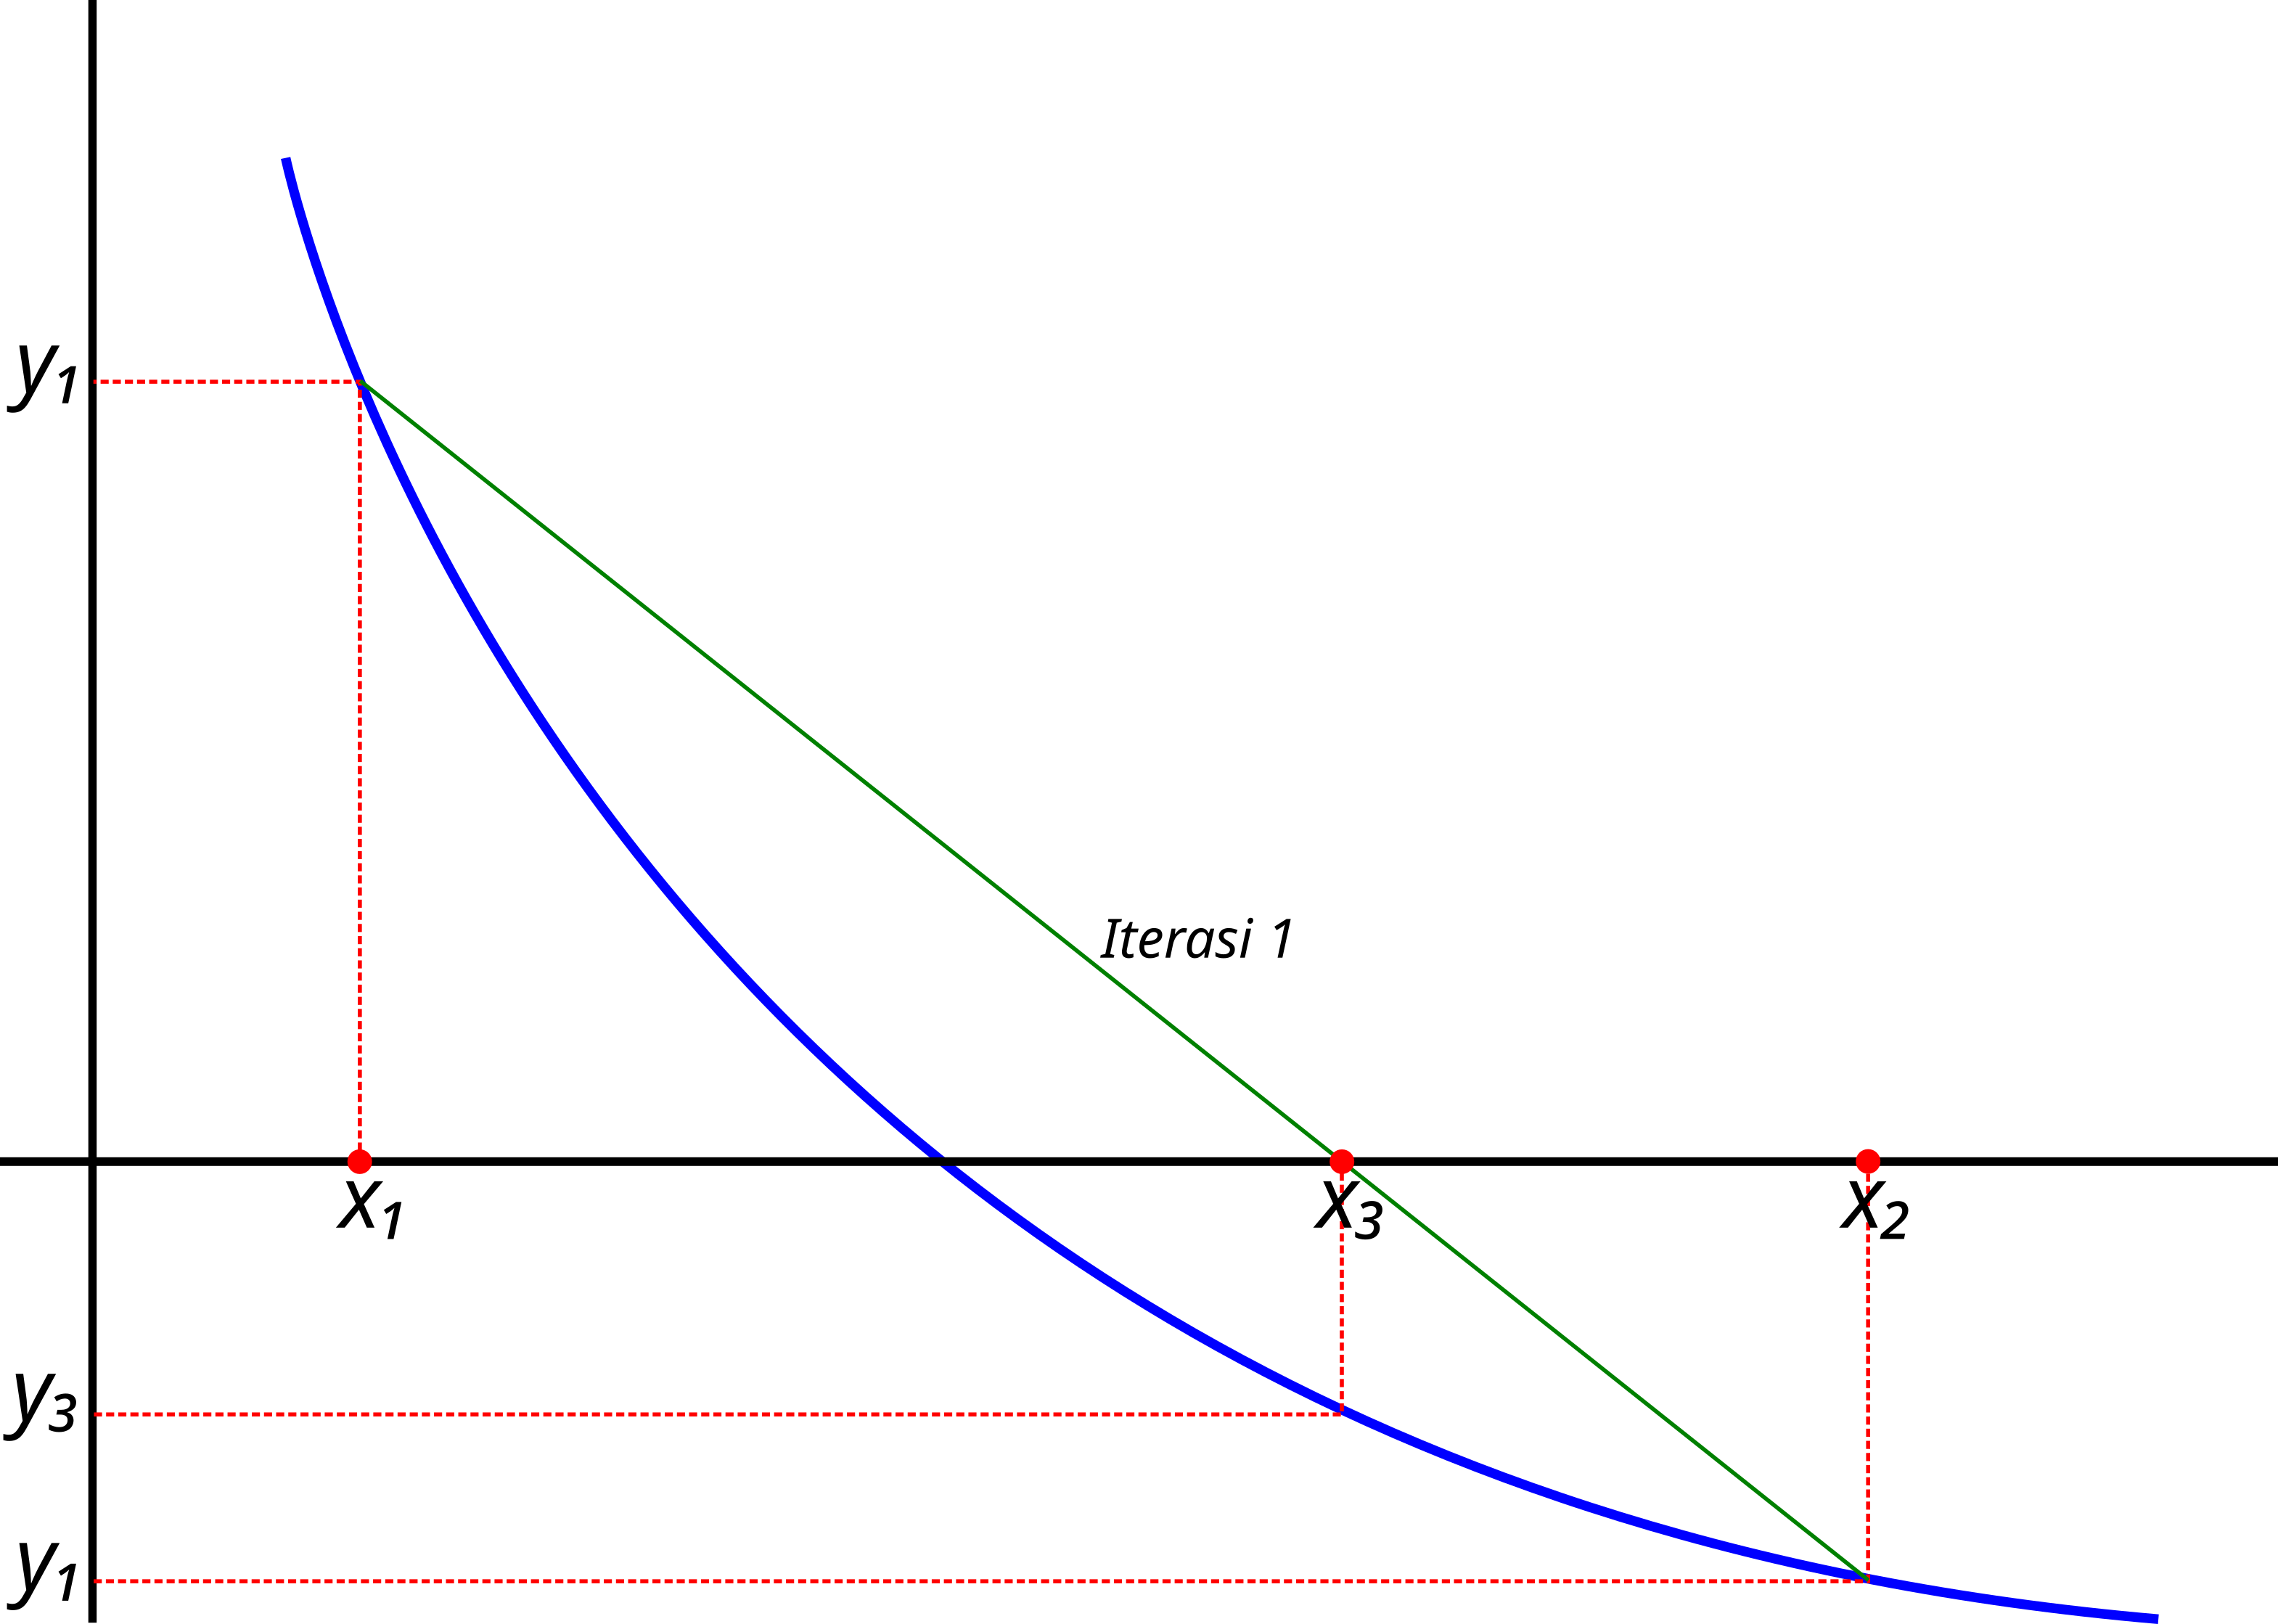
\includegraphics[width=0.7\linewidth]{img/04}
	\end{center}
	$$ x_3 = x_{2} - \frac{x_{2}-x_{1}}{y_{2}-y_{1}}y_{2} $$
\end{frame}

\begin{frame}{Metode Secant}
	\begin{center}
		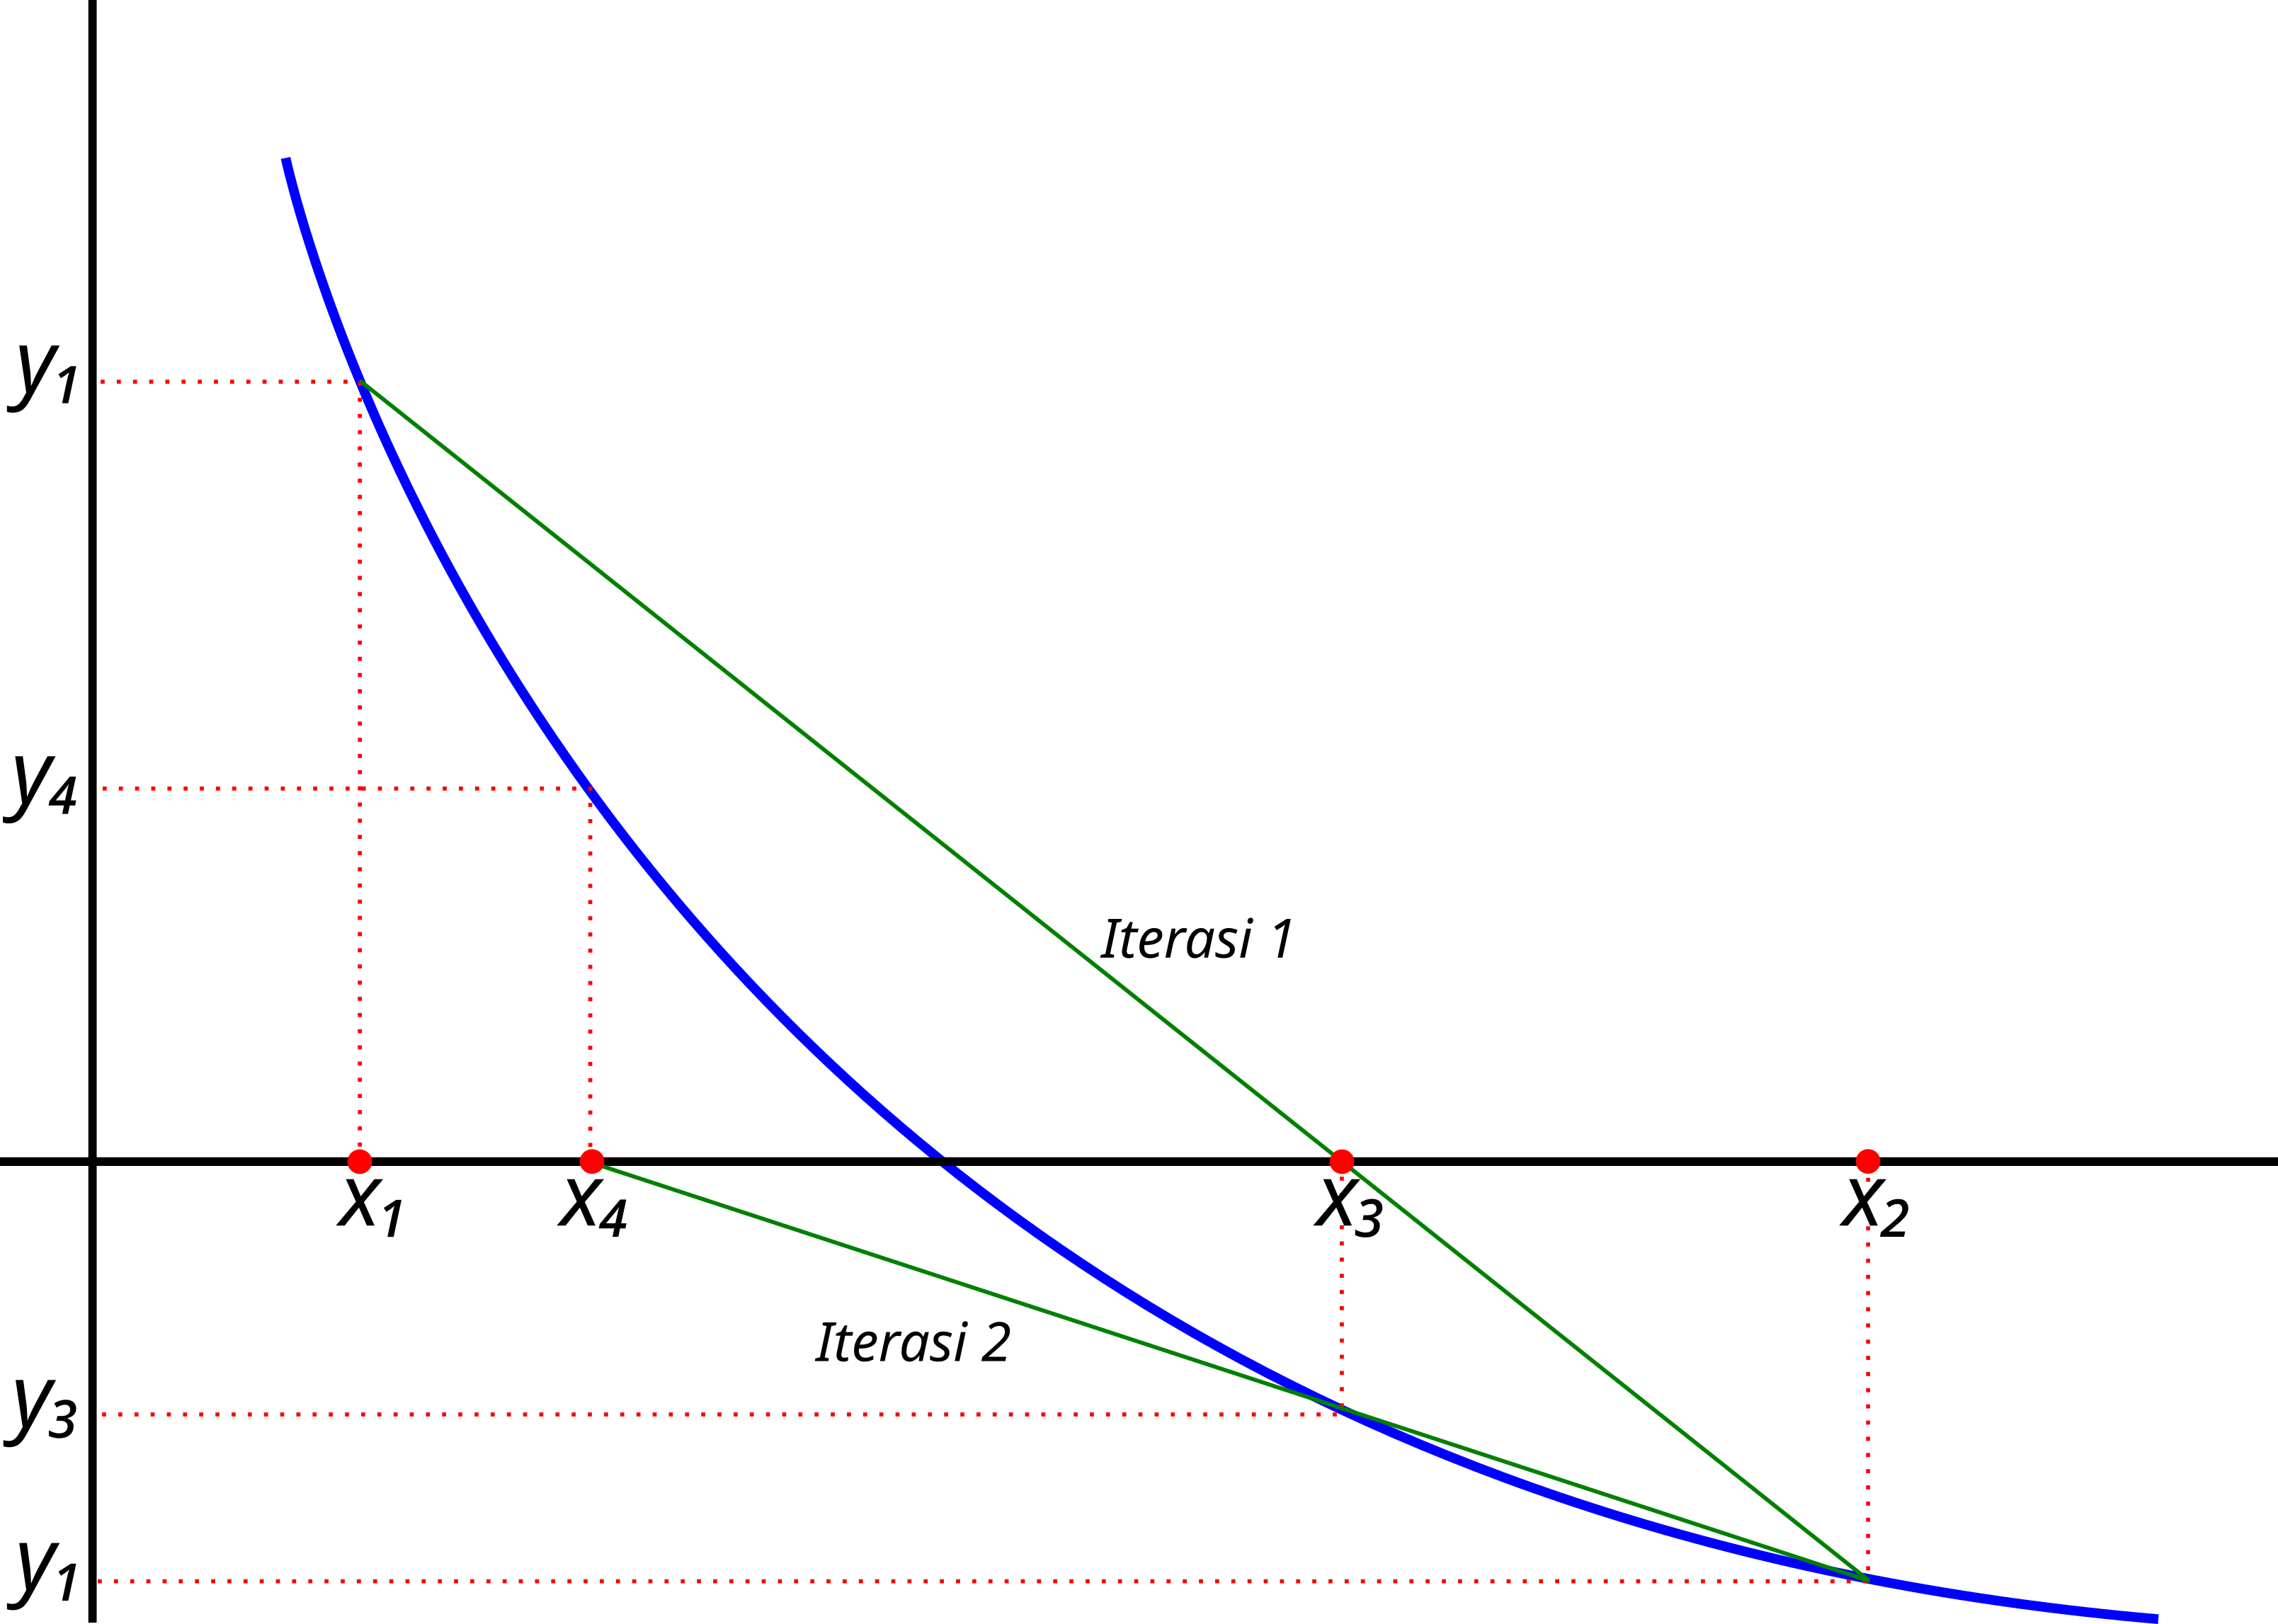
\includegraphics[width=0.7\linewidth]{img/05}
	\end{center}
	$$ x_4 = x_{3} - \frac{x_{3}-x_{2}}{y_{3}-y_{2}}y_{3} $$
\end{frame}

\begin{frame}
	\frametitle{Contoh 5}
	Tentukan akar-akar dari persamaan $$ 2x^2 - 5x + 3 = 0 $$ dengan menggunakan metode Secant.
\end{frame}

\section{Tugas 1}

\begin{frame}
	\frametitle{Tugas 1}
	\begin{enumerate}
		\item Jelaskan mengapa seorang \textit{electrical engineer} membutuhkan metode numerik? Sertakan contoh kasus yang ada di dunia \textit{electrical engineer} yang diselesaikan dengan menggunakan metode numerik/ analisis numerik.
		\item Tahun 1225, Leonardo da Pisa mencari akar persamaan
		$$ f(x) = x^3 + 2x^2 + 10x - 20 = 0 $$
		dan menemukan $ x = 1.368808107 $. Tidak seorang pun yang mengetahui cara
		Leonardo menemukan nilai ini. Jelaskan prosedur apa yang digunakan untuk mendapatkan  akar persamaan yang ditemukan Leonardo itu.
	\end{enumerate}
\end{frame}

\end{document}
